\chapter{Introduction}

\section{Problem Statement}

 STEM (science, technology, engineering, and math) fields are a primary focus in education, because there is increasing need for students who have the technical skills to solve real-world problems. A major challenge that many STEM educators face is engaging students in the classroom. The education technology (ed-tech) startup, SE3D, hopes to solve this challenge by bringing 3D bioprinting technology to high school classrooms. Although SE3D has already produced a working prototype, the printer only has basic capabilities and requires further development.  

The 3D bioprinter senior design team aims to create a 3D bioprinter that can improve the capabilities of high school teachers to engage students in STEM education. Implementing 3D bioprinters into high schools will generate increased understanding and interest in biology, research, and technology for the students who will soon be America’s doctors, technicians, and scientific pioneers. 

In order to accomplish this goal, the team is expanding SE3D’s product line to improve student and teacher user experiences and to expand the possibilities for biological experiments. Table \ref{table:problem-solution} shows how SE3D’s current printer can be improved to meet these goals. 

\begin{table}[H]
\caption{\label{table:problem-solution} Current Bioprinter Problems and Senior Design Project Solutions}

\begin{tabularx}{\textwidth}{ |X|X| }
  \hline
  \textbf{Problem }& \textbf{Solution }\\

  \hline 
Printer lacks advanced features: automated camera, temperature control and humidity regulation

- Limits capability of experimentation

&  

Develop a separate, modular incubation unit (The Box) with an automated camera and humidity and temperature controls

- Analysis and printing can occur in parallel since functions are not in same physical space

- Automatic image capture to analyze experiment over time

- Simple user interface to configure and run experiments
 \\


    \hline 
 Printer only prints with one material

- Limits print designs
  & 
  Design and implement low cost dual extruder
   \\
  \hline
  Motion control system relies on specialized 3D printer software and feature-limited hardware

- Duet Control Board only supports basic 3D printing operations

- External computer necessary for control
&
Create custom software environment
- Distributed control board system to accommodate extra control features
Run on built-in computer 

- Keep low-cost with Raspberry Pi 

\\
  \hline
  Operator must manually calibrate syringe extruder

- Room for human error
&
Implement auto-calibration software of the syringe extruder
\\
  \hline
\end{tabularx}

\end{table}


The goals in Table \ref{table:problem-solution} are subject to the following criteria:
\begin{enumerate}
	\item Usable in a high school lab environment by both students and teachers
	\item Safe for all users
	\item Low cost
\end{enumerate}

% =======================================================================

% =======================================================================
\section{Background and Related Work}

The current bioprinter produced by SE3D, the r3bEL, is marketed towards high school science classes. It prints using a single 5 mL syringe that has to be manually loaded by the user, put into the head of the bioprinter, and calibrated by hand to begin printing. It currently has the capability to print enzyme, alga, and bacterium 2D arrays, chocolate, and cells and scaffolds for 3D tissue engineering. The r3bEL printer can print four 3x3 array tray experiments in about 3 minutes. After it is finished, the experiment must remain on the bed of the bioprinter until it finishes culturing. The user gathers data form the experiment by constantly taking pictures of the experiment as it cultures. To capture more consistent and higher quality images, an SE3D employee created a separate box that block out external light and has its own light source. This small box has a removable ceiling, lined with LEDs, and holds a single Petri dish. A small hole in the ceiling allows a mobile phone camera to be placed over it to capture images of the experiment as it cultures, though it still requires an individual to operate the camera and capture each image.


\begin{table}[H]
\caption{\label{table:printer-comparison} Comparison of Existing 3D Bioprinters}
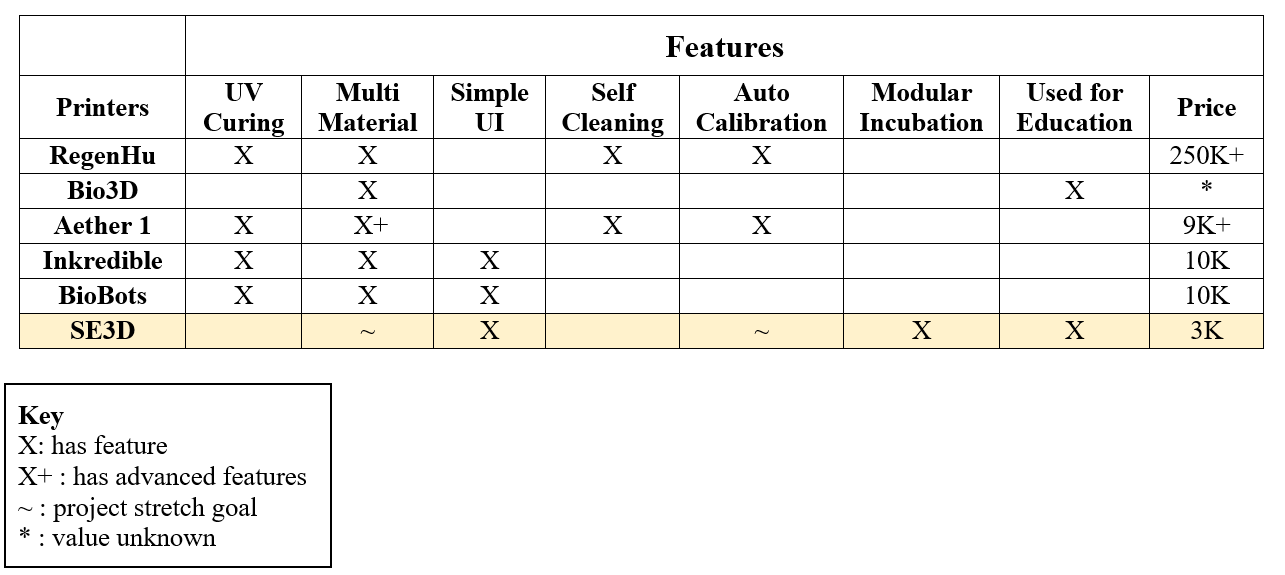
\includegraphics{printer-comparison-table}
\end{table}
Although the team is enhancing the functionality of SE3D’s 3D Bioprinter, there are currently many similar products that are already available for purchase. Below are the bioprinters shown in Table \ref{table:printer-comparison} with an explanation of their key features and price ranges.



\textit{RegenHu: 3D Discovery Printer} \\
RegenHu produces a professional printer priced at 250,000+ USD. It supports a wide range of funcationalities and applications. It is primarily used for optimal processing of a broad biomaterial/bioactives portfolio. The device prints using cell-friendly Ink-jet and thermopolymer extrusion using a 2-component printhead. In addition, it has a high precision temperature controller for biomaterial culturing.

\textit{Bio3D Technologies: Bio3D Explorer Series}\\
Three-dimensional bioprinters have also been developed internationally. Bio3D Technologies in Singapore has a series of printers in their Explorer product line. Designed for educational purposes, the Bio3D has 1 to 4 printing heads available and is lightweight and foldable with a full metal frame. The device is suitable for a wide range of applications and materials. The price was not listed online.

\textit{Aether 1 3D Bioprinter} \\
Aether has a 3D bioprinter that begins with a base unit cost of 9,000 USD. The product includes 8 syringes, 2 hot ends, and 10 extruder print heads. It has the widest range of usable materials for printing, from oils to plastics. The device has many useful attachments, like a UV curing light for biomaterial prints. Its extruders are pneumatic-driven.

\textit{CellInk: Inkredible Printer} \\
In Palo Alto, California, CellInk manufactures a research grade bioprinter, Inkredible. Inkredible is priced at 10,000 USD for the base version of the printer. It focuses on assisting tissue engineers who use their custom bioink line to create hydrogel structures that allow for efficient mammalian cell culturing. It has been optimized to print skin and cartilage tissue and uses UV lighting to cure the biomaterial. The printer has a clean chamber and heated cartridges.

\textit{BioBots 3D Printer} \\
BioBots has a desktop 3D printer capable of printing tissues out of living cells. The base model price of BioBots’ 3D printer is 10,000 USD. It is small and portable to allow for ease of use. In addition, the device has a dual heated, pneumatic driven extruder system for precise printing and uses replaceable syringes for easy material changing. Blue light technology is used to safely cure the biomaterial. BioBots is based in Philadelphia; however, they ship internationally.

After reviewing these printers, it is clear that they are all capable of completing the biological experiments that SE3D desires. The one aspect that they all do not meet, however, is that they are priced much higher than the average high school laboratory budget. Furthermore, these printers require high levels of knowledge in order to operate, which is not a reasonable expectation of high school students. To improve this aspect, the UI must be simplified and easy to use for people with less than a high school education. The closest competitors are Inkredible and BioBots, which are low cost and have simple user interfaces. The 3D Bioprinter that the team is working on improves on this problem by providing the necessary functionality at a more reasonable price closer to 3,000 USD. 

% =======================================================================
\section{Literature Review}

The 3D Bioprinter project hopes to assist SE3D, a stem education and 3D Bioprinting company, in the development of their newest 3D bioprinter model. This project has been ongoing for several years, with the intention of improving upon the existing prototype, based on the company’s needs. 
\\
\textbf{Incubation Methods}
\\
When dealing with biological matter, the environment in which the material is placed must be carefully controlled. For this reason, part of the project objective is to explore possible mechanisms for monitoring temperature, humidity, and lighting during an experiment. Time is an important element for running lessons, and the printer may need to be used multiple times. In order to accommodate this, this project hopes to design an external incubator. The incubation system will be controlled using a microcontroller and must be low cost; these criteria drove primary research for the incubator.
\\
\textit{Ibrahim’s Low Cost Temperature Controllers}
\\
Ibrahim used micro-controllers to develop a low cost temperature control unit. His research illustrates how the temperature in a heat exchanger can be controlled with a micro-controller that controls the amount of radiation given off by the unit.  Since our projects focuses on the affordability of the Bioprinter for high schools, this method for temperature control demonstrates a way to keep the price low while still completing the temperature control criteria. This experimental procedure will be followed and further tested to determine how best to control the air surrounding the heat source, such that the entire incubation chamber temperature can be within a few degrees.
\\
\textbf{Z-axis and Multiple Material Printing}
\\
One focus of this project is to improve the system’s ability to print biomaterials in the third dimension. Currently, the printer is primarily used for 2D science experiments and utilizes a single extruder syringe to print experiments. This single syringe needs to be manually replaced if it runs out or if a new material is being printed. This project aims to implement a dual extruder to streamline the printing process and to enhance the structural capabilities of the printed materials, such that printing in the z-axis direction is less restricted. Research gathered on printers with multiple extruders will assist in understanding the ideal methods for efficiently printing multiple materials and printing in the z-axis direction.
\\
\textit{Ozbolat’s Multi-arm Bioprinter}
\\
The multi-arm bioprinter developed in 2014 created a method for printing two biological materials without manually replacing or exchanging the extruder source. Two fully independent robotic arms controlled the position, ejection speed, and temperature of the nozzle of each material. The single-arm multi-material test that was run by Ozbolat’s team required that the flow of the biological material was controlled externally from the robotic arm. Ozbolat’s lab ran tests using sodium alginate and calcium chloride, the same substances used for one of SE3D’s experiments; however, SE3D’s bioprinter has only one robotic arm to eject the biomaterial. The single-arm extruder method provides a base understanding of how to eject both materials from a single arm while still taking into account varying viscosity and temperature needs. 
\\
\textit{Gao’s Coaxial Nozzle Method}
\\
The 3D printer developed by Gao experimented with different flow rates and material concentrations to determine the optimum high strength printable biological material. The printer used an interchangeable coaxial nozzle to print the hollow cavity of the filament. This allowed the experimenters to control the inside diameter without significantly altering the outside diameter. SE3D’s bioprinter uses a single nozzle in the form of a syringe, which has made it difficult to print complex physical structures. Gao’s research differs from the mission of the project in that method for printing multiple materials is not restricted to a coaxial nozzle. However, the experimentation and successful creation of complex 3D structures using multiple materials is vital to the understanding of how to successfully implement true 3D printing. 
\\
\textbf{Software Redesign}
\\
The final design requirement requested by SE3D is improving the 3D printer control software system. The open source software that the system currently uses will be replaced by a new custom software environment that will create a simple GUI for the average high school student user. However, it will also be extensible to control all of the supplementary features that will be added in the redesign. This software environment will run on a built-in computer, making the printer a stand alone device. In order to develop this system, research must be conducted to understand the general software structure of a 3D printer.
\\
\textit{Rankin and OctoPrint}
\\
Previous processes for printing a 3D object involved generating a 3D model in STL format, converting the STL file to GCODE using a slicing software, then using a communication software, such as Pronterface, to load the GCODE and send it to the printer. What is problematic with using software like Pronterface is it needs to be run from an external computer that needs to be connected to the 3D printer at all times, which is the design SE3D currently uses. Rankin recommends a software called OctoPrint that runs the 3D printer control software on a web interface, so printing is controlled and monitored over the network and can be run off of a Raspberry Pi. Operating over the network allows for the potential to connect more control boards to the main interface, which allows more room to control the additional features planned for the printer.

% =======================================================================

\section{Objectives}

The 3D bioprinting team consists of mechanical engineers, computer engineers, and bioengineers. To accomplish the project goals, the team has split the project into three parts: The Box, 3D Printing Feasibility Study, and a bioengineering experiment. The bulk of this document will focus on the software components for The Box and 3d Printing feasibility study, as that will be where the computer engineering work is applied.
\begin{itemize}
	\item  The Box:
	\begin{enumerate}
		\item Meet with Maya, SE3D CEO to define requirements for the incubating box
		\item Make design decisions for functionality included in the box and physical and structural designs
		\item Develop prototypes of box, user interface, and controls, allowing users to customize the box environment, begin and end experiments, and automatically capture a series of photos
		\item At every stage of development, run tests for proper software and hardware compatibility
		\item Share prototype with users in a classroom setting for feedback
	\end{enumerate}
	\\
	\item 3D Printer Feasability Study:
	\begin{enumerate}
		\item Analyze usability of the SE3D bioprinter and identify areas of improvement.

		\item Incorporate an auto-calibration mechanism for the syringe plunger though physical designs and adaptation of printer firmware.

		\item Extend printer functionality to two extruders for multi-material extrusion of biomaterial and the other PLA.

		\item At every stage of development, run tests for proper software and hardware compatibility.

		\item Share prototypes with stakeholders for feedback.
	\end{enumerate}
\end{itemize}